\documentclass[a4paper,10pt]{article}
%\documentclass[a4paper,10pt]{scrartcl}

\usepackage[fleqn]{amsmath}
\usepackage{amsfonts}
\usepackage{amssymb}
\usepackage[utf8]{inputenc}
\usepackage{tabularx}
\usepackage{mathtools}
\usepackage{tikz}
\usetikzlibrary{positioning}

\renewcommand{\tabularxcolumn}[1]{m{#1}}

\title{Discorn Protocol Motivation and Documentation}
\author{Suwako Moriya}
\date{2021}

\pdfinfo{%
  /Title    (Discorn Protocol Documentation)
  /Author   (SuwakoMmh)
  /Creator  (SuwakoMmh)
  /Producer (SuwakoMmh)
  /Subject  (Cryptography)
  /Keywords ()
}

\begin{document}
    \maketitle
    \tableofcontents
    \section{Why ?}
        Computers bring with them a new problem : It has become hard to get forgotten.
        Anything one shares with a company over the internet is potentially stored forever and used against them.
        Malicious entities such as hypothetical future governments might use such data against part of the population
        and endanger democracy.\\
        
        We defend a basic right to privacy and we are going to claim it no matter what thanks to cryptography.
        Bitcoin has opened the way with a trustless consensus protocol used in a currency. But the same idea
        can be used in many other applications. Discorn is a protocol that aims to achieve what apps such as Discord did,
        with the bonus of being open-source and decentralized.\\
        
        
        Examples of encrypted or decentralized messaging apps exists but we dislike the centralized nature of some of them
        and the federated nature of others. To put it simply:
        \begin{itemize}
         \item We dislike centralized software because it creates a single point of failure that governments can control
         if they please and because it relies on trust of a single third party.
        
        \item And we dislike federated software as well because it is a hassle to create a local instance : it requires web-related
         knowledge, a domain name, and the hardware to make it run. If one doesn't want to create a local instance because of all of that,
         then he has to trust a third party for his privacy. Which could be worse than the centralized alternative in some cases.
         We have been lead towards Matrix when our first ideas of Discorn emerged and yes, it does allow for chatting channels, VoIP and some kind of Guildish features.
         However we believe that we can do better both in usability and privacy.
        \end{itemize}
        The end-user, when using Discorn, not only helps claim a future for Humanity and get his privacy back. He also wins the freedom
        of free software. Discorn can be modded, and nobody will be banned by Discorn. Because Discorn is no more than a protocol.
    
    \section{Structure}
        Discorn is organised around Guilds. A Guild is a network of people sharing a Blockchain, it is created by one individual that
        can either claim its ownership or leave the Guild in anarchy. Being the owner of a Guild means having permission to promote
        new administrators, creating discussion channels, choosing who can join the network, moderating the messages and tweak other parameters.
        In an anarchist Guild, everyone has every right.
        

    \section{Blockchain}
    
        \subsection{Block}
            To be valid, a block's hash must begin with a certain number of zeros. \\
            Let $X$ be the number of random hashes to mine a block with difficulty $d$, $X$ follows a geometric distribution : $Geo(\frac{1}{2^d})$. Hence : $\mathbb{E}(X)= 2^d$
            
            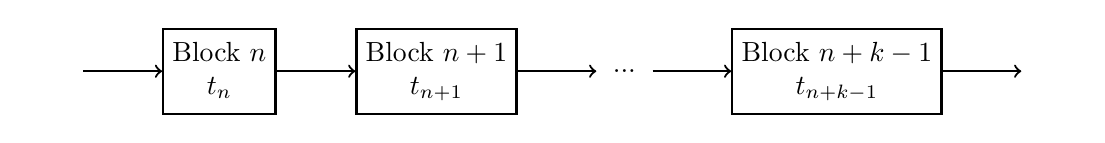
\begin{tikzpicture}[blocknode/.style={rectangle, draw=black, thick, minimum size=7mm},
                                floatingnode/.style={rectangle, minimum size=7mm},]
                \node[floatingnode] (0) {};
                \node[blocknode] (1) [right=of 0] {$\begin{matrix}\text{Block $n$}\\t_n\end{matrix}$};
                \node[blocknode] (2) [right= of 1] {$\begin{matrix}\text{Block $n+1$}\\t_{n+1}\end{matrix}$};
                \node[floatingnode] (3) [right= of 2] {...};
                \node[blocknode] (4) [right= of 3] {$\begin{matrix}\text{Block $n+k-1$}\\t_{n+k-1}\end{matrix}$};
                \node[floatingnode] (5) [right= of 4] {};
                \draw[thick,->] (0.east) -- (1.west);
                \draw[thick,->] (1.east) -- (2.west);
                \draw[thick,->] (2.east) -- (3.west);
                \draw[thick,->] (3.east) -- (4.west);
                \draw[thick,->] (4.east) -- (5.west);
            \end{tikzpicture}\\
            
            Let $\Delta t$ be the average time interval between two blocks over a $k$ blocks interval.
            
            \begin {align*}
             \Delta t = \frac{t_{n+k-1} - t_n}{k}
            \end {align*}

            
            To estimate the network's hashrate $N$ $[hash.s^{-1}]$, we use the following expression\\
            
            \begin {align*}
                &\text{}N = \frac{k\mathbb{E}(X)}{\Delta t} = \frac{k2^d}{\Delta t}\\
                &\text{We can express the next difficulty with ${\Delta t}_{target}$ and $k$}\\
                &N = \frac{k2^{d_{next}}}{{\Delta t}_{target}}\\
                &\Leftrightarrow 2^{d_{next}} = \frac{N{\Delta t}_{target}}{k}\\
                &\Leftrightarrow d_{next} = \left\lfloor\log_2\left(\frac{{\Delta t}_{target}}{k}\right)\right\rfloor
            \end {align*}\\
            \begin{tabularx}{\textwidth}{|l|l|X|l|}
            \hline Field & Type & Description & Length \\ \hline
            \hline Version & big-endian int & Block version & 1 byte \\
            \hline Timestamp & big-endian int & & 4 bytes\\
            \hline Corner count & big-endian int & Number of Corner included & 3 bytes\\
            \hline Merkle root & cryptonote-fast-hash & Root hash of Corners Merkle tree & 32 bytes\\
            \hline Previous hash & cryptonote-slow-hash & Hash of previous block & 32 bytes\\
            \hline Difficulty & big-endian int & The calculated difficulty target being used for this block & 4 bytes\\
            \hline Nonce & raw & To allow variations of the header and compute different hashes & 4 bytes \\
            \hline
            \hline Coinbase & Corner & Special Corner that has outputs without inputs & \\
            \hline Corners & Corner list & Corners one after the other & \\
            \hline
            \end{tabularx}
        
        \subsection{Corner}
           \begin{tabularx}{\textwidth}{|l|l|X|l|}
            \hline Field & Type & Description & Length \\ \hline
            \hline Payload length & big-endian int &  & 3 bytes \\
            \hline Payload flag ($P_{Flag}$) & big-endian int &  & 1 byte \\
            \hline Payload & raw & & \\
            \hline
            \end{tabularx}
            \subsubsection{Transaction (Tx) :  $P_{Flag} = 0$}
                \begin{tabularx}{\textwidth}{|l|l|X|l|}
                \hline Field & Type & Description & Length \\ \hline
                \hline Version & big-endian int & Tx version & 1 byte \\
                \hline Input count & big-endian int & Number of Inputs included & 3 bytes\\
                \hline Input Puzzles & Input list & Transaction's inputs & \\
                \hline Output count & big-endian int & Number of Outputs included & 3 bytes\\
                \hline Output Puzzles & Puzzle list & Transaction's outputs & \\
                \hline Solutions & Solution list & To unlock each input, a Challenge has to be solved. & \\
                \hline
                \end{tabularx}
            \subsubsection{Event : $P_{Flag} = 1$}
                \begin{tabularx}{\textwidth}{|l|l|X|l|}
                \hline Field & Type & Description & Length \\ \hline
                \hline Version & big-endian int & Event version & 1 byte \\
                \hline Hash & cryptonote-fast-hash & Event hash as in the event database & 32 Bytes\\
                \hline Authorization & Auth & Proof that the Event is legitimate & \\
                \hline
                \end{tabularx}
        \subsection{Input (Tx)}
           \begin{tabularx}{\textwidth}{|l|l|X|l|}
            \hline Field & Type & Description & Length \\ \hline
            \hline Payload length & big-endian int &  & 3 bytes \\
            \hline Payload flag ($P_{Flag}$) & big-endian int &  & 1 byte \\
            \hline Payload & raw & & \\
            \hline
            \end{tabularx}
        \subsection{Puzzles \& Solutions (Tx)}
           \begin{tabularx}{\textwidth}{|l|l|X|l|}
            \hline Field & Type & Description & Length \\ \hline
            \hline Payload length & big-endian int &  & 3 bytes \\
            \hline Payload flag ($P_{Flag}$) & big-endian int &  & 1 byte \\
            \hline Payload & raw & & \\
            \hline
            \end{tabularx}
            \subsubsection{}

    \section{Networking}
\end{document}
